\documentclass[8pt, twoside]{extarticle}

\usepackage[
	twocolumn,
	left=0.8in,
	right=0.8in,
	top=1.2in,
	bottom=1.3in
]{geometry}

\linespread{1.07}
\usepackage[skip=5pt]{parskip}

\usepackage[hidelinks]{hyperref}
\usepackage{amsmath} 
\usepackage{amsfonts} 
\usepackage{xcolor}

\usepackage [english]{babel}
\usepackage [autostyle, english = american]{csquotes}
\MakeOuterQuote{"}


\usepackage{breakcites}


\makeatletter
\renewcommand*{\verbatim@font}{\ttfamily\small}
\makeatother


\usepackage{fancyhdr}
\setlength{\headheight}{15pt}

\pagestyle{fancy}
\renewcommand{\headrulewidth}{0pt}
\renewcommand{\footrulewidth}{0pt}

\makeatletter
\fancyhf{}
\fancyhead[LE]{\thepage\ · \small\smallauthor}
\fancyhead[RO]{\small\@title\normalsize\ · \thepage}
\fancyfoot[LE,RO]{\small Publication date: \today}
\makeatother


\usepackage{caption}
\captionsetup[lstlisting]{font={small}}


\renewcommand{\arraystretch}{1.1}


\usepackage{listings}
\lstdefinestyle{default}{basicstyle=\ttfamily\small, commentstyle=, columns=flexible, keepspaces=true, tabsize=2, breaklines=true, breakatwhitespace=true, numbers=left, numberstyle=\tiny, xleftmargin=5mm, captionpos=t}
\lstset{style=default}


\usepackage{tikz}
\tikzstyle{arrow} = [-latex]

\usepackage{qtree}
\newcommand{\qlabelhook}{\small}


\usepackage{pgfplots}
\usepackage{pgfplotstable}


\makeatletter\renewcommand\maketitle{{
	{\Huge\@title }\\[4ex] 
	{\Large\@author\normalsize, \affiliation}\vspace{\baselineskip}
}}\makeatother


\title{Developing Grammar Fuzzers}
\author{Aarush Kumbhakern}
\def\smallauthor{Kumbhakern}
\def\affiliation{Ashoka University, India}


\setlength{\columnsep}{20pt}


\begin{document}

\thispagestyle{empty}

\maketitle

\begin{abstract}
	\small

	Fuzzing is used for testing the resiliency of programs to input-based attacks. Fuzzers prioritize two key aspects - effectiveness in identifying vulnerabilities and the efficiency or speed at which they operate. While random fuzzers are exceptionally fast, their efficiency is hindered by input parsing challenges. In contrast, grammar fuzzers achieve deeper code penetration by generating specification conforming output.

    This paper describes the development and optimization of a suite of grammar fuzzers. The paper includes comprehensive exploration of several fuzzing techniques, emphasizing efficiency through performance testing. Additionally, the paper delves into specific insights relevant to C language development and explores potential novel approaches to enhance existing fuzzer sub-processes.
\end{abstract}


\section{Introduction}

Fuzzing is a method used to test the resiliency of programs against unexpected, malformed, or malicious user input, by generating and injecting large amounts/iterations of such input. An example of a simple fuzzer is a random string generator. However, the majority of programs that take user input have input parsers to validate the input against a program-specific input language (e.g. a CSS minifier likely first checks if the input text is in fact valid CSS). In most instances, a randomly generated string would fail at this initial validation stage, and would be largely ineffective in testing deeper program logic. To reach program internals beyond the parser, a fuzzer must generate inputs that follow the grammar of the program's input language - such a fuzzer is termed a generation-based or grammar fuzzer \cite{Felderer_2016}. 

\subsection{Grammars}

A grammar consists of definitions (e.g. \verb|"<start>": [...]|), which in turn consist of rules (e.g. \verb|["<expr>"]|), which then in turn consist of symbols/tokens (e.g. \verb|"<expr>"|) \cite{Salem_2019}. A grammar contains two types of symbols:

\begin{enumerate}
	\item \textbf{Terminal:} single ASCII characters, that when encountered are directly written to the fuzzer's output. Termed as such due to the fact that they "terminate" the expansion

	\item \textbf{Nonterminal:} demarcated by surrounding angled brackets (\verb|<...>|), each corresponding to a definition. Nonterminals are heuristically expanded into any of the corresponding definition's rules
\end{enumerate}

The \verb|<start>| token (or some alias) must exist in any grammar, and is the starting point of the expansion of a grammar. Listing \ref{lst:arithmetic_grammar} shows a JSON grammar that defines an arithmetic expression.

\begin{lstlisting}[gobble=2, caption={Arithmetic expression grammar}, label=lst:arithmetic_grammar]
	{
		"<start>": [
			["<expr>"]
		],
		"<expr>": [
			["<term>", "+", "<expr>"],
			["<term>", "-", "<expr>"],
			["<term>"]
		],
		"<term>": [
			["<factor>", "*", "<term>"],
			["<factor>", "/", "<term>"],
			["<factor>"]
		],
		"<factor>": [
			["+", "<factor>"],
			["-", "<factor>"],
			["<integer>", ".", "<integer>"],
			["<integer>"]
		],
		"<integer>": [
			["<digit>", "<integer>"],
			["<digit>"]
		],
		"<digit>": [
			["0"], ["1"], ["2"], 
			["3"], ["4"], ["5"], 
			["6"], ["7"], ["8"], 
			["9"]
		]
	}
\end{lstlisting}

\subsection{Expansion}

A grammar fuzzer, at its core, automates the expansion of a given grammar by stochastically expanding nonterminal tokens based on their corresponding definitions. Listing \ref{lst:simple_fuzzer} shows pseudocode for a simple grammar fuzzer.

\begin{lstlisting}[gobble=2, caption={Simple grammar fuzzer pseudocode}, label=lst:simple_fuzzer]
	def fuzz(grammar):
		fuzz = "<start>"

		while not fully_expanded(fuzz):
			for token in fuzz:
				if nonterminal(token):
					expansion = expand(token, grammar)
					fuzz.replace(token, expansion) 

		return fuzz
\end{lstlisting}

Listing \ref{lst:expansion_example} describes an example expansion trace of the arithmetic grammar, where each step expands all nonterminal tokens in the preceding step.

\begin{lstlisting}[gobble=2, caption={Arithmetic grammar expansion}, label=lst:expansion_example]
	<start>
	<expr>
	<term>
	<factor>
	<integer>.<integer>
	<digit>.<digit><integer>
	8.1<digit>
	8.12
\end{lstlisting}

A notable issue with the simplistic approach in Listing \ref{lst:simple_fuzzer} is the lack of control over expansion depth. Many grammars feature recursive rules, and without proper control, a simple grammar fuzzer may become ensnared in an infinite expansion loop. Moreover, even reaching a sufficiently large expansion depth can have adverse effects on a recursive fuzzer, especially when constrained by a fixed stack size.

Beyond this challenge, the primary concern in simple fuzzing lies in speed (measured in terms of throughput in Kb/s, or output size over time), which is essential as a fuzzer is expected to rapidly generate either single inputs of considerable size or a substantial number of inputs of varying sizes.

\subsection{Outline}

After briefly describing evaluation standards and methods and providing hardware specifications of the test machine (Section \ref{sec:hardware}), this paper is organized as follows:

\paragraph{Section \ref{sec:excntflw}} We briefly discuss recursive and iterative approaches to how a fuzzer might handle expansion of a grammar.

\paragraph{Section \ref{sec:limexdpth}} We discuss various methods to control expansion depth specific to each control flow approach, with a specific focus on creating a mechanism to maintain a "current depth" state.

\paragraph{Section \ref{sec:genfuzz}} We create iterative and recursive variants of grammar-agnostic generic fuzzers, and discuss the construction of grammar structures for use with generic fuzzers.

\paragraph{Section \ref{sec:compfuzz}} We create Python compilers to compile an input grammar into C program code, condensing the generic fuzzers' runtime grammar evaluation into a single compilation step to achieve significant increases in efficiency. We also discuss for the first time methods to algorithmically break recursive rings to generate cheap grammars.

\paragraph{Section \ref{sec:profiling}} We benchmark each fuzzer variant described in this paper according to a set of standards, and compare and discuss differences in performance statistics

\section{Evaluation and Hardware} \label{sec:hardware}

All fuzzers are evaluated on the basis of throughput in Kb/s. 

All fuzzers achieve seeded output parity, ie. for a given seed value, all fuzzer variants will generate the same fuzzed string. Fuzzers will therefore be evaluated on their average performance at various depths for a fixed set of 10 randomly generated seeds.

The development and testing machine is a Zephyrus G14 (2021) running Fedora Linux on an AMD Ryzen 5800HS 8-core processor with a 2.8 GHz frequency, 512kb L2 cache, and 16MB shared L3 cache.

\section{Expansion Control Flow} \label{sec:excntflw}

This section explores recursive and iterative approaches to the core fuzzing process of fully expanding a grammar - going from \verb|<start>| to a fuzzed output string.

\subsection{Recursive Expansion} \label{sec:recexp}

Figure \ref{fig:recursive_expansion_tree} represents lines 4 to 8 of the example expansion in Listing \ref{lst:expansion_example} as a tree.

\begin{figure}[hbt!]
	\Tree[ .Factor [ .Integer [ .Digit "8" ] ] "." [ .Integer [ .Digit "1" ][ .Integer [ .Digit "2" ] ] ] ]

	\caption{Recursive expansion tree}
	\label{fig:recursive_expansion_tree}
\end{figure}

Consider each nonterminal node to be a call to a \verb|fuzz()| function (e.g. "Digit" is \verb|fuzz(digit)|), and each terminal leaf to be the action of \verb|print()|-ing that terminal token to the fuzzer's output. Here, \verb|fuzz()| writes terminals to the output with and generates recursive calls to \verb|fuzz()| for each nonterminal token in the selected expansion. Listing \ref{lst:recursive_expansion_pseudocode} shows the static (pseudocode) function body of the Factor node in Figure \ref{fig:recursive_expansion_tree} (note that this function body is specific to this particular call to \verb|fuzz()|).

\begin{lstlisting}[gobble=2, caption={Recursive expansion pseudocode fragment}, label=lst:recursive_expansion_pseudocode]
	fuzz(factor):
		fuzz(integer)
		print(".")
		fuzz(integer)
\end{lstlisting}

\subsection{Iterative Expansion} \label{sec:iterative_expansion}

Consider the definition of \verb|expr| in the arithmetic grammar in \ref{lst:arithmetic_grammar}. Two rules in this definition are self-referential, implying a recursive call to the fuzzer as seen in the previous section. Starting from \verb|expr|, if each subsequent \verb|expr| token in the expansion is expanded into a self-referencing rule, this will eventually lead to stack exhaustion as a result of a large number of recursive calls.

To address specifically the concern of a limited stack size, an alternative iterative approach can be adopted, wherein the program explicitly manages its own stack. In our pure iterative expansion method, the fuzzer iteratively mutates a \textit{production string} or \textit{expansion stack}. Table \ref{tbl:iterative_expansion} shows the iterative version of the same detailed expansion described in Figure \ref{fig:recursive_expansion_tree}.

\begin{table}[hbt!]
	\centering\small

	\begin{tabular}{ll}
		 Stack                                                & Out  \\
		 \hline % ------------------------------------------------------
		 $\langle$factor$\rangle$                             &      \\
		 $\langle$integer$\rangle$.$\langle$integer$\rangle$  &      \\
		 $\langle$digit$\rangle$.$\langle$integer$\rangle$    &      \\
		 8.$\langle$integer$\rangle$                          &      \\
		 .$\langle$integer$\rangle$                           & 8    \\
		 $\langle$integer$\rangle$                            & 8.   \\
		 $\langle$digit$\rangle$$\langle$integer$\rangle$     & 8.   \\
		 1$\langle$integer$\rangle$                           & 8.   \\
		 $\langle$integer$\rangle$                            & 8.1  \\
		 $\langle$digit$\rangle$                              & 8.1  \\
		 2                                                    & 8.1  \\
		                                                      & 8.12
	\end{tabular}

	\caption{Iterative Expansion}
	\label{tbl:iterative_expansion}
\end{table}

Observe that the number of steps in the expansion (excluding the pre-iteration first step) corresponds to the number of nodes in the recursive expansion tree (Figure \ref{fig:recursive_expansion_tree}).

It is essential to note that the fuzzer exclusively operates on the head of the expansion stack, writing to the fuzzer's output if the token is a terminal and substituting it with an expansion if the token is a nonterminal. Listing \ref{lst:iterative_expansion_pseudocode} shows pseudocode for the iterative expansion approach.

\begin{lstlisting}[gobble=2, caption={Iterative expansion pseudocode}, label=lst:iterative_expansion_pseudocode]
	def fuzz(stack):
		while length(stack) > 0:
			head, remainder = stack
			
			if terminal(head):
				print(head)
				stack = remainder

			else:
				stack = expand(head) + remainder
\end{lstlisting}

\subsection{A Common Approach} \label{sec:comapp}

After examining the explicit expansion steps outlined in the iterative expansion (Table \ref{tbl:iterative_expansion}) and comparing them to the recursive tree representation of the same expansion (Figure \ref{fig:recursive_expansion_tree}), we observe that the expansion process follows an approach analogous to a depth-first left-to-right scan of the expansion tree. Notably, this approach is consistent across all fuzzers presented in this paper.

\section{Limiting Expansion Depth} \label{sec:limexdpth}

Referring again to the tree in Figure \ref{fig:recursive_expansion_tree}, the term \textit{expansion path} will hereafter refer to a series of contiguous nodes (e.g. \verb|factor| $\rightarrow$ \verb|integer| $\rightarrow$ \verb|digit| $\rightarrow$ \verb|"1"|) with reference to a single origin node. 

Depth also is visually represented by the vertical position of tokens in the tree. If we consider \verb|factor| to start at depth 1, both \verb|digit| tokens, for example, are at a depth of 3 in their expansion paths.

\subsection{Approach Overview} \label{sec:limdepapov}

It is more accurate to term expansion depth as \textit{free} expansion depth, ie. the expansion depth up to which the fuzzer is entirely uninhibited in its expansion of nonterminal tokens. Once an expansion path grows to a certain maximum expansion depth $\mu$, the fuzzer adopts an approach of selecting exclusively non-recursive ("cheap") rules to continue the path. This renders any token $x$ s.t $\text{depth}(x)=\mu$ functionally terminal. 

To illustrate, consider $\mu=1$ and Figure \ref{fig:expansion_subtree}, which frames a subtree of the expansion tree in Figure \ref{fig:recursive_expansion_tree}.

\begin{figure}[hbt!]
	\Tree[ .Factor [ .Integer [ .Digit "8" ] ] "." [ .Integer [ .Digit "1" ] [ .Integer [ .Digit "2" ] ] ] !{\qframesubtree} ]
	
	\caption{Depth-limiting candidate}
	\label{fig:expansion_subtree}
\end{figure}

Assuming \verb|factor| is at a depth of 0, the first \verb|integer| in the subtree is observed at a depth of 1 ($\ge \mu$) in the expansion path. Consequently, a depth-limited grammar fuzzer would exclusively choose "cheap" rules from the definition of \verb|integer| to continue the expansion. The annotated definition of \verb|integer| from the arithmetic grammar (Listing \ref{lst:arithmetic_grammar}) in Listing \ref{lst:annotated_definition} highlights the cheap and expensive rules.

\begin{lstlisting}[gobble=2, language=Python, caption={Annotated integer Definition}, label=lst:annotated_definition]
	"<integer>": [
		["<digit>", "<integer>"],   # (expensive)
		["<digit>"]                 # (cheap)
	],
\end{lstlisting}

By assigning appropriate costs to each rule, only one possible expansion of \verb|integer| remains, accordingly simplifying the framed subtree in Figure \ref{fig:expansion_subtree} into the subtree in Figure \ref{fig:simplified_subtree}.

\begin{figure}[hbt!]
	\Tree[ .Integer [ .Digit "0..9" ] ]
	
	\caption{Limited subtree}
	\label{fig:simplified_subtree}
\end{figure}

Thus, to successfully limit expansion depth, two key requirements must be addressed:

\begin{enumerate}
	\item Maintaining a "current depth" state specific to the fuzzer's position in the current expansion pathway
	\item Separately identifying cheap and expensive rules
\end{enumerate}

At present we will assume manual identification and separation of rules by cost, and consider only direct recursion, ie. self-referencing rules. The paper will further explore this aspect of depth-limiting in Section \ref{sec:chpgram}, where we will algorithmically determine whether a rule is cheap or expensive, and additionally identify indirect recursion in grammars. 

This section will focus solely on maintaining the "current depth" state of a fuzzer.

\subsection{Recursive Limiting} \label{sec:reclim}

The fact that a recursive approach explicitly constructs a tree makes maintaining a "current depth" state trivial. The process becomes straightforward as we only need to increment an argument for subsequent function calls, ie. \verb|fuzz(x, depth)| $\rightarrow$ \verb|fuzz(y, depth + 1)|. Figure \ref{fig:reclimtree} demonstrates by modifying the tree in Figure \ref{fig:recursive_expansion_tree}.

\begin{figure}[hbt!]
	\Tree[ .{fuzz(factor, 0)} [ .{fuzz(integer, 1)} [ .{fuzz(factor, 2)} \small print("8") ] ] \small print(".") !\qsetw{0cm} [ .{fuzz(integer, 1)} [ .{fuzz(digit, 2)} \small print("1") ][ .{fuzz(integer, 2)} [ .{fuzz(digit, 3)} \small print("2") ] ] ] ]

	\caption{Recursive expansion tree}
	\label{fig:reclimtree}
\end{figure}

Listing \ref{lst:recursive_limiting_pseudocode} shows the modified function body of the Factor node.

\begin{lstlisting}[gobble=2, caption={Recursive depth parameter}, label=lst:recursive_limiting_pseudocode]
	fuzz(factor, depth):
		fuzz(integer, depth + 1)
		print(".")
		fuzz(integer, depth + 1)
\end{lstlisting}

\subsection{Iterative Limiting} \label{sec:iterlim}

Maintaining a depth state for a pure iterative expansion approach is considerably more complex due to the implicit nature of the expansion, and the fact that the fuzzer just runs a loop which in itself provides no useful depth state. 

Our solution uses a combination of a "history" array \verb|stc| (Stepwise Token Count), and a (current) \verb|depth| state variable. The history array acts as a step-wise token count, with each index corresponding to a specific depth in the expansion path. Simultaneously, the current depth state variable dynamically tracks the depth during the iterative process.

\subsubsection{Incrementing Depth}

Incrementing depth is trivial - every time the iterative fuzzer encounters a nonterminal, we increment \verb|depth|. We will begin constructing a stripped-down implementation of only the limiting portion of the code in C:

\begin{lstlisting}[gobble=2, language=C, caption={Rudimentary depth increment}]
	while (STACK_LEN > 0) {
		if(token >= 0) { // if terminal
			continue;
		}

		depth++;
	}
\end{lstlisting}

\subsubsection{Maintaining Token Count History}

The key to figuring out when to decrement depth, is knowing when the expansion of a token in the current expansion path at a given depth is resolved, ie. all tokens in the expansion have been evaluated. This critical task is facilitated by the history array (\verb|stc|).

Every time the fuzzer encounters a nonterminal, before prepending the nonterminal's expansion to the production string, the token count of the expansion is written to the history array, and the current depth is then incremented as discussed above:

\begin{lstlisting}[gobble=2, language=C, caption={Writing token count to memory}]
	while (STACK_LEN > 0) {
		if(token >= 0) { // if terminal
			continue;
		}

		// record token count then increment depth
		stc[depth++] = rule->token_count;
	}
\end{lstlisting}

\subsubsection{Evaluating Tokens}

Every iteration of the fuzzer corresponds to the evaluation of a single token, underscoring the granularity of the iterative expansion process. In this context, with each iteration, the number of un-evaluated tokens in the expansion of the token at \verb|depth - 1| is systematically decremented:

\begin{lstlisting}[gobble=2, language=C, caption={Every loop is an evaluation}]
	while (STACK_LEN > 0) {
		// decrement latest token count
		if (depth > 0) stc[depth - 1]--;

		if(token >= 0) { // if terminal
			continue;
		}

		// record token count then increment depth
		stc[depth++] = rule->token_count;
	}
\end{lstlisting}

\subsubsection{Resolving Expansions}

We recognize that a token is fully resolved only when the final terminal in its expansion is encountered. To illustrate, consider Figure \ref{fig:parrestree}:

\begin{figure}[hbt!]
	\Tree[ .foo "a" [ .bar "b" "c" ] ]

	\caption{Partial resolution example}
	\label{fig:parrestree}
\end{figure}

In this example, \verb|foo| is partially resolved when the fuzzer moves on to \verb|bar| as all the tokens in the current expansion of \verb|foo| have been evaluated. However, \verb|foo| achieves complete resolution only upon encountering the final terminal of its full expansion \verb|"c"|.

A fundamental understanding emerges: a nonterminal will always increase the depth, and only a terminal can signal a decrease in depth. Even if a token becomes fully resolved by the evaluation of token $x$, if $x$ is a nonterminal, decreasing the depth would be premature. We therefore check for resolution only upon encountering a terminal. Listing \ref{lst:rescheck} demonstrates the resolution check:

\begin{lstlisting}[gobble=2, language=C, caption={Checking for resolution}, label=lst:rescheck]
	while (STACK_LEN > 0) {
		// decrement latest token count
		if (depth > 0) stc[depth - 1]--;

		if(token >= 0) { // if terminal
			// rollback to nearest unresolved
			while (stc[depth - 1] == 0) depth--;
			
			continue;
		}

		// record token count then increment depth
		stc[depth++] = rule->token_count;
	}
\end{lstlisting}

In this code snippet, the check for resolution is placed in a conditional \verb|while| loop. This design ensures that complete resolution cascades down through any preceding partial resolutions. For instance, in the expansion of \verb|foo|, encountering \verb|"c""| marks not only \verb|bar| as resolved but cascades down through the partial resolution of \verb|foo|, marking it as completely resolved as well.

\subsubsection{Accounting for Limiting}

As we introduce limiting, the logic of the depth state mechanism undergoes a slight modification. Recall that any token $x$ at the maximum depth $\mu$ becomes functionally terminal due to the limiting. Consequently, at this point, the depth state mechanism focuses solely on whether $x$ has been fully resolved. Any expansions or sub-expansions of $x$ are flattened, and depth updates are temporarily paused.

This adjustment in the depth state mechanism reflects the shift in focus when limiting is introduced. The mechanism now prioritizes the determination of full resolution for tokens at the maximum depth, simplifying the expansion process during this specific phase.

\begin{lstlisting}[gobble=2, language=C, caption={Complete depth state maintenance mechanism}]
	while (STACK_LEN > 0) {
		// decrement latest token count
		if (depth > 0 && depth < max_depth) stc[depth - 1]--;

		if(token >= 0) { // if terminal
			// if haven't already, decrement latest token count
			if (depth > 0 && depth >= max_depth) stc[depth - 1]--;
			
			// rollback to nearest unresolved
			while (stc[depth - 1] == 0) depth--;
			
			continue;
		}

		// record token count then increment depth
		if (depth < max_depth) stc[depth++] = rule->token_count;
		else stc[depth - 1] += (rule->token_count) - 1;
	}
\end{lstlisting}

\subsubsection{Example Execution}

Table \ref{tbl:iterative_depth_state} shows an example of the iterative depth state mechanism in action, using the iterative expansion example in Section \ref{sec:iterative_expansion}.

\begin{table}[hbt!]
	\centering\small

	\begin{tabular}{clll}
		Depth & \verb|stc[]|                     & Stack                                                & Out  \\
		\hline % --------------------------------------------------------------------------------------------------
		0     & []                              & $\langle$factor$\rangle$                             &      \\
		1     & [3]                            & $\langle$integer$\rangle$.$\langle$integer$\rangle$  &      \\
		2     & [2,1]                          & $\langle$digit$\rangle$.$\langle$integer$\rangle$    &      \\
		3     & [2,0,1]                        & 8.$\langle$integer$\rangle$                          &      \\
		1     & [2,0,0] $\rightarrow$ [2]    & .$\langle$integer$\rangle$                           & 8    \\
		1     & [1]                            & $\langle$integer$\rangle$                            & 8.   \\
		2     & [0,2]                          & $\langle$digit$\rangle$$\langle$integer$\rangle$     & 8.   \\
		3     & [0,1,1]                        & 1$\langle$integer$\rangle$                           & 8.   \\
		2     & [0,1,0] $\rightarrow$ [0,1]  & $\langle$integer$\rangle$                            & 8.1  \\
		3     & [0,0,1]                        & $\langle$digit$\rangle$                              & 8.1  \\
		4     & [0,0,0,1]                      & 2                                                    & 8.1  \\
		0     & [0,0,0,0] $\rightarrow$ []    &                                                      & 8.12
	\end{tabular}

	\caption{Iterative Depth State Mechanism}
	\label{tbl:iterative_depth_state}
\end{table}

\section{Generic Fuzzers} \label{sec:genfuzz}

A generic fuzzer is a function that takes a grammar defined in a certain predefined structure as an input, and produces a fuzzed output that conforms to said grammar. Evaluation and expansion of the grammar are both runtime processes.

In this section we construct recursive and iterative variants of a generic fuzzer in C. We will begin by defining the structure for the input grammar. 

\subsection{Grammar Structure}

We first declare the components that will comprise the grammar - tokens, rules, and definitions - and a simple structure for the grammar itself:

\begin{lstlisting}[gobble=2, language=C, caption={Generic grammar components}]
	typedef signed char token_t;

	typedef struct Rule {
		size_t token_count;
		token_t* tokens;
	} Rule;

	typedef struct Definition {
		size_t rule_count[2];
		Rule* rules[2]; // [0]: cheap, [1]: costly
	} Definition;

	typedef struct Grammar {
		Definition* definitions;
	} Grammar;
\end{lstlisting}

The \verb|struct| components are self-explanatory, but it is worth clarifying with regard to the \verb|rules| member in \verb|Definition| that \verb|rule[0]| contains the definition's cheap rules, and \verb|rule[1]| contains its expensive rules. 

The \verb|typedef| for tokens is specifically of type \verb|signed char| as we will be representing terminals with their corresponding (positive) ASCII codes, and nonterminals with negative values - this allows identifying nonterminals to be simplified to a trivial arithmetic inequality test. The way these negative values are assigned is as follows (using the arithmetic grammar (Listing \ref{lst:arithmetic_grammar}) as an example):

\begin{lstlisting}[gobble=2, language=C, caption={Defining nonterminals}] 
	enum nonterminals {start = SCHAR_MIN, expr, term, factor, integer, digit};
\end{lstlisting}

The \verb|start| token is assigned the lowest possible negative value, and each key in the grammar is automatically assigned the next lowest value in order of appearance in the \verb|enum|. The value of each key is then tied to the index of its corresponding definition in the final grammar using designated initializers.

\begin{lstlisting}[gobble=2, language=C, caption={Generic grammar snippet}]
	Grammar grammar = {.definitions=(Definition []) {
		[start - start] = (Definition) { // start
			.rule_count={1, 0}, 
			.rules={
				(Rule []) { // "<rule>"
					(Rule) { 
						.token_count=1, 
						.tokens=(token_t[]) {expr} 
					},
				},
			} 
		},
		
		[expr - start] = (Definition) { // expr
			.rule_count={1, 2}, 
			.rules={
				(Rule []) {
					(Rule) { // "<term>"
						.token_count=1, 
						.tokens=(token_t[]) {term} 
					},
				},
				(Rule []) {
					(Rule) { // "<term>+<expr>"
						.token_count=3, 
						.tokens=(token_t[]) {term, '+', expr} 
					},
					(Rule) { // "<term>-<expr>"
						.token_count=3, 
						.tokens=(token_t[]) {term, '-', expr} 
					},
				},
			} 
		},

		// ...and so on
	} };
\end{lstlisting}

\subsection{Recursive Generic Fuzzer}

\subsubsection{Making Recursive Calls}

In the recursive expansion trees we have seen so far, tokens are directly expanded via recursive calls into a chosen expansion, ie. for \verb|<x>| $\rightarrow$ \verb|<a>+<b>|, we would generate the pseudocode in Listing \ref{lst:recgenpsd1}.

\begin{lstlisting}[gobble=2, language=C, caption={Recursive expansion}, label=lst:recgenpsd1] 
	fuzz(x):
		fuzz(a)
		print("+")
		fuzz(b)
\end{lstlisting}

However, actual implementation requires the fuzzer to first select a rule and then, depending on the type of token, make recursive sub-calls or write to output for each nonterminal in the expansion, all within a loop, as shown in Listing \ref{lst:recgenpsd2}.

\begin{lstlisting}[gobble=2, language=C, caption={Realistic evaluation}, label=lst:recgenpsd2] 
	fuzz(x):
		rule = get_rule(x) // [a, "+", b]

		for token in rule:
			if rule is terminal: print(token)
			else: fuzz(token)
\end{lstlisting}

Listing \ref{lst:recgenpsd3} shows the logic up to this point translated into C.

\begin{lstlisting}[gobble=2, language=C, caption={Rudimentary implementation}, label=lst:recgenpsd3] 
	fuzzer(Grammar* grammar, token_t token) {
		Definition* def = &grammar->definitions[token - start];
		Rule* rule = get_rule(def)

		for (size_t i = 0; i < rule->token_count; i++) {
			// if terminal write to stdout
			if (rule->tokens[i] >= 0) {
				putchar(rule->tokens[i]);
			} else { // otherwise make recursive call
				fuzzer(grammar, rule->tokens[i]);
			}
		}
	}
\end{lstlisting}

We will discuss the actual implementation of \verb|get_rule()| in section \ref{sec:selrule} below - for now, we simply assume that it returns a random rule from the definition passed to it.

\subsubsection{Limiting Depth}

Limiting depth for a recursive, as discussed, is primarily an issue of rule selection and depth state maintenance. 

We will assume that \verb|get_rule(token, cheap)| will choose only cheap rules if \verb|cheap = 1|. 

The condition for switching to an exclusively cheap rule selection mode is \verb|depth >= max_depth|. \verb|max_depth| can be passed in as a static parameter, and as discussed in Section \ref{sec:reclim} depth may be simply passed as an argument for a recursive fuzzer. Listing \ref{lst:recgenfuzzcmp} shows the updated recursive fuzzer.

\begin{lstlisting}[gobble=2, language=C, caption={Depth-limited generic recursive fuzzer}, label=lst:recgenfuzzcmp] 
	fuzzer(Grammar* grammar, depth_t max_depth, depth_t depth, token_t token) {
		Definition* def = &grammar->definitions[token - start];
		Rule* rule = get_rule(def, depth >= max_depth)

		for (size_t i = 0; i < rule->token_count; i++) {
			// if terminal write to stdout
			if (rule->tokens[i] >= 0) {
				putchar(rule->tokens[i]);
			} else { // otherwise make recursive call
				fuzzer(grammar, max_depth, depth + 1, rule->tokens[i]);
			}
		}
	}
\end{lstlisting}

An additional check has been added to ensure that the fuzzer does not attempt to choose expensive rules if the current token’s definition does not contain any. 

This completes the generic recursive fuzzer implementation.

\subsubsection{Selecting Rules} \label{sec:selrule}

The \verb|get_rule()| function chooses a random rule from a given definition. If \verb|cheap = 1|, it chooses only cheap rules.

\begin{lstlisting}[gobble=2, language=C, caption={Get rule function}] 
	Rule* get_rule(Definition* definition, int cheap) {
		size_t cheap_c = definition->rule_count[0];
		size_t exp_c = definition->rule_count[1];
		
		// force cheap if no expensive rules
		if (!exp_c) cheap = 1;

		if (cheap) {
			return &definition->rules[0][rand() % cheap_c];
		
		} else {
			// choose from cumulative rule set
			size_t choice = rand() % (cheap_c + exp_c);
			size_t cost = choice >= cheap_c;
			if (cost) choice -= cheap_c;
			return &definition->rules[cost][choice];
		}
	}
\end{lstlisting}

\subsection{Iterative Generic Fuzzer}

\subsubsection{Iterative Expansion}

To summarize the approach described in Section \ref{sec:iterative_expansion}, a pure iterative fuzzer mutates an expansion stack by iteratively evaluating the first token in the stack - writing it to output if terminal and expanding it if nonterminal.

We will again begin by minimally implementing an iterative fuzzer that conforms to this description.

\begin{lstlisting}[gobble=2, language=C, caption={Simple generic iterative fuzzer}] 
	void fuzzer(Grammar* grammar) {
		token_t* stack = malloc(1024 * sizeof(token_t));
		stack[0] = start; // initialize stack with start

		size_t stack_len = 1;

		while (stack_len > 0) {
			token_t token = stack[0]; // get first token

			// if token is terminal write to stdout
			if (token >= 0) {
				// remove token from stack
				memmove(stack, stack + 1, --stack_len);
				
				putchar(token);

				continue;
			}
			
			Definition* def = &grammar->definitions[token - start];
			Rule* rule = get_rule(def);

			// substitute token with rule in stack 
			memmove(stack + rule->token_count, stack + 1, stack_len * sizeof(token_t));
			memcpy(stack, rule->tokens, rule->token_count);
			stack_len += rule->token_count - 1;
		}
	}
\end{lstlisting}

The iterative fuzzer shares the implementation of its \verb|get_rule()| function with the recursive fuzzer (Section \ref{sec:selrule}).

\subsubsection{Limiting Depth}

As it happens, we have already discussed everything needed to implement depth limiting in the iterative fuzzer. With the understanding that we are using the same \verb|get_rule()| function, we can simply copy the internal rule choice code from the recursive fuzzer, and then merge the iterative depth limiting mechanism from Section \ref{sec:iterlim} with the current code for the fuzzer:

\begin{lstlisting}[gobble=2, language=C, caption={Depth-limited generic iterative fuzzer}] 
	void fuzzer(Grammar* grammar, depth_t max_depth) {
		token_t* stack = malloc(1024 * sizeof(token_t));
		stack[0] = start; // initialize stack with start

		size_t stack_len = 1;

		// depth state variables
		depth_t stepwise_token_count[128] = {};
		depth_t current_depth = 0;

		while (stack_len > 0) {
			token_t token = stack[0]; // get first token
			
			// decrement latest token count
			if (depth > 0 && depth < max_depth) stc[depth - 1]--;

			// if token is terminal write to stdout
			if (token >= 0) {
				// remove token from stack
				memmove(stack, stack + 1, --stack_len);

				putchar(token);

				// if haven't already, decrement latest token count
				if (depth > 0 && depth >= max_depth) stc[depth - 1]--;
							
				// rollback to nearest unresolved token
				while (stc[depth - 1] == 0) depth--;

				continue;
			}
			
			Definition* def = &grammar->definitions[token - start];
			Rule* rule = get_rule(def, depth >= max_depth)

			// record token count then increment depth
			if (depth < max_depth) stc[depth++] = rule->token_count;
			else stc[depth - 1] += (rule->token_count) - 1;

			// substitute token with rule in stack 
			memmove(stack + rule->token_count, stack + 1, stack_len * sizeof(token_t));
			memcpy(stack, rule->tokens, rule->token_count);
			stack_len += rule->token_count - 1; 
		}
	}
\end{lstlisting}

This completes the generic iterative fuzzer.


\section{Compiled Fuzzers} \label{sec:compfuzz}

To reiterate, generic fuzzers perform two major runtime processes:

\begin{enumerate}
	\item Evaluate the input grammar
	\item Expand the \verb|start| token in a manner defined by the input grammar to create fuzzed output
\end{enumerate}

This section aims to enhance fuzzer speed by consolidating the runtime evaluation of the input grammar into a single compilation step. The approach involves compiling a given grammar into program code specific to that grammar.

Since the compilation is a one-time activity and not a runtime process, speed is not a primary concern. For convenience, the compiler and its utilities will be implemented in Python but will output program code in C.

Moreover, this section will not delve into the details of the compiler's implementation but will instead concentrate on the expected output of the compiler. The compiler program will produce a C module, comprising a header file and an implementation file. However, our focus in this section will be solely on the implementation file.

\subsection{Generalized Pseudo-Implementation} \label{sec:genpsimp}

\subsubsection{Basic Compilation}

The compilation process is straightforward. Definitions are transformed into functions, rules are selected by conditional matching with a randomly generated number within the range of the definition’s rule count, and each token in a rule is converted into a call to the corresponding definition if nonterminal, or a write function if terminal.

Consider the example in Listing \ref{lst:compexpsd1} of the compilation of \verb|expr| from the arithmetic grammar (Listing \ref{lst:arithmetic_grammar}) into pseudocode.

\begin{lstlisting}[gobble=2, caption={Example compilation (pseudocode)}, label=lst:compexpsd1]
	expr():
		choice = random(3)

		if choice == 0:
			term()
			print("+")
			expr()

		if choice == 1:
			term()
			print("-")
			expr()

		if choice == 2:
			term()
\end{lstlisting}

\subsubsection{Limiting Depth}

A compiled fuzzer uses the same recursive approach to depth state maintenance as discussed in Section \ref{sec:reclim}. Actual limiting via cheap rule section is achieved by compiling two variants - cheap and random - for each definition. When the fuzzer reaches a maximum depth, the random variant will redirect to the cheap variant.

\begin{lstlisting}[gobble=2, language=Python, caption={Compiled fuzzer depth limiting}]
	# cheap variant
	expr_cheap():
		choice = random(1)

		if choice == 0:
			term_cheap()


	# random variant
	expr_rand(max_depth, depth):
		if depth >= max_depth: # redirect to cheap
			expr_cheap()
			return

		choice = random(3)

		if choice == 0:
			term_rand(max_depth, depth + 1)
			print("+")
			expr_rand(max_depth, depth + 1)

		if choice == 1:
			term_rand(max_depth, depth + 1)
			print("-")
			expr_rand(max_depth, depth + 1)

		if choice == 2:
			term_rand(max_depth, depth + 1)
\end{lstlisting}

Tokens in the rules of the cheap variant of a generator only redirect in turn to the cheap generators of said tokens, ie. once the fuzzer switches to using a cheap generator, it exclusively uses cheap generators for the remainder of the expansion path.

The cheap variants are generated from a cheap sub-grammar of the original grammar. The next section will discuss how cheap grammars are generated.

\subsection{Cheap Grammar Generation} \label{sec:chpgram}

A cheap grammar is a sub-grammar that contains only cheap (non-recursive) rules. The central operation in the cheapening of a grammar, and the focus of this section, lies in the identification and pruning of recursive rules. Up until now, the paper has assumed the manual identification and separation of cheap and expensive rules. However, it is imperative for us to develop the capability to algorithmically identify recursive rules in grammars.

\subsubsection{Indirect Recursion} \label{sec:indrec}

Up to this point, we have been exposed only to direct (self-referential) recursion. We will now broaden our definition of recursive rules to include indirect recursion. Consider the "perfidious" grammar in Listing \ref{lst:prfgram}.

\begin{lstlisting}[gobble=2, caption={Perfidious grammar}, label=lst:prfgram]
	{
		"<start>": [
			["<foo>"],
			["a"] 
		],
		"<foo>": [
			["<bar>"],
			["b"]
		],
		"<bar>": [
			["<baz>"],
			["<start>"],
		],
		"<baz>": [
			["(", "<foo>", ")"],
			["c"],
		]
	}
\end{lstlisting}

The grammar contains no direct recursion, but further examination reveals two recursive "rings":

\begin{figure}[hbt!]
	\centering
	
	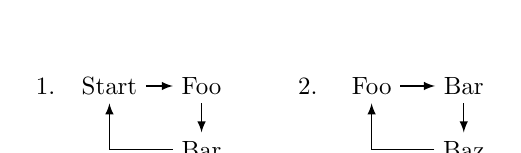
\begin{tikzpicture}[node distance=0.9cm, every node/.style={scale=0.9}]
		\node (start) {Start};
		\node (1enum) [left of=start] {1.};
		\node (1foo) [right of=start, xshift=0.4cm] {Foo};
		\node (1bar) [below of=1foo] {Bar};
		
		\draw [arrow] (start) -- (1foo);
		\draw [arrow] (1foo) -- (1bar);
		\draw [arrow] (1bar) -| (start);
		
		\node (2foo) [right of=1foo, xshift=1.5cm] {Foo};
		\node (2enum) [left of=2foo] {2.};
		\node (2bar) [right of=2foo, xshift=0.4cm] {Bar};
		\node (2baz) [below of=2bar] {Baz};
		
		\draw [arrow] (2foo) -- (2bar);
		\draw [arrow] (2bar) -- (2baz);
		\draw [arrow] (2baz) -| (2foo);
	\end{tikzpicture}

	\caption{Perfidious grammar rings}
	\label{fig:prfgramrings}
\end{figure}

Our goal is to identify and break these rings, ie. ensure no such rings exist in the cheap grammar.

\subsubsection{Cheapening approaches} \label{sec:chpapp}

There are two approaches to cheapening a grammar.

In a \textbf{permissive} approach, a rule is retained as long as the number of non-recursive expansion pathways is $>1$, even all other expansion pathways are recursive. A permissive approach will only remove "vicious" rings, ie. rings that cannot be terminated without completing a full circuit. In other words, this approach will remove a rule if \textit{all} expansion paths from said rule lead back to itself:

This means that rings may still exist in the grammar - for example, a permissive approach would not remove any of the rings in the recent perfidious grammar (Listing \ref{lst:prfgram}). This undermines the purpose of cheapening to the end of limiting depth, and does not conform to our "functionally terminal" (Section \ref{sec:limdepapov}) requirement. Consequently, we proceed to explore the next approach.

In broad terms, an \textbf{aggressive} approach adopts a more stringent criterion by removing any rule that causes recursion. There are two sub-approaches to identifying the cause of a ring. To illustrate, consider Figure \ref{fig:prfgramexp} - the expansion path diagram for the perfidious grammar (Listing \ref{lst:prfgram}).

\begin{figure}[hbt!]
	\centering

	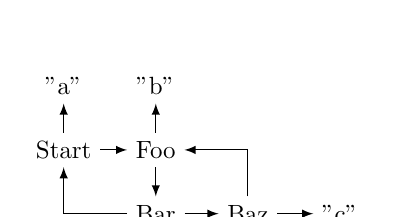
\begin{tikzpicture}[node distance=0.9cm, every node/.style={scale=0.9}]
		\node (end1) {"a"};
		\node (start) [below of=end1] {Start};
		\node (foo) [right of=start, xshift=0.4cm] {Foo};
		\node (end2) [above of=foo] {"b"};
		\node (bar) [below of=foo] {Bar};
		\node (baz) [right of=bar, xshift=0.4cm] {Baz};
		\node (end3) [right of=baz, xshift=0.4cm] {"c"};
		
		\draw [arrow] (start) -- (end1);
		\draw [arrow] (start) -- (foo);
		\draw [arrow] (foo) -- (end2);
		\draw [arrow] (foo) -- (bar);
		\draw [arrow] (bar) -| (start);
		\draw [arrow] (bar) -- (baz);
		\draw [arrow] (baz) |- (foo);
		\draw [arrow] (baz) -- (end3);
	\end{tikzpicture}

	\caption{Perfidious grammar expansion map}
	\label{fig:prfgramexp}
\end{figure}

The first sub-approach would attribute recursion to the point of entry to a ring. In this \textbf{head-first} approach, we iterate over every rule in the grammar and prune it if we find any expansion paths leading from the rule that form a ring (i.e., the rule is an entry point).

Consider ring 1 in Figure \ref{fig:prfgramrings}, the entry points to which could be either \verb|start| $\rightarrow$ \verb|foo| or \verb|foo| $\rightarrow$ \verb|bar|. Figures \ref{fig:ringentryex1} and \ref{fig:ringentryex2} show the effects of pruning these entry points.

\begin{figure}[hbt!]
	\centering

	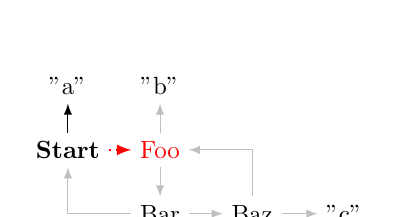
\begin{tikzpicture}[node distance=0.9cm, every node/.style={scale=0.9}]
		\node (end1) {"a"};
		\node (start) [below of=end1] {\textbf{Start}};
		\node (foo) [right of=start, xshift=0.4cm, text=red] {Foo};
		\node (end2) [above of=foo] {"b"};
		\node (bar) [below of=foo] {Bar};
		\node (baz) [right of=bar, xshift=0.4cm] {Baz};
		\node (end3) [right of=baz, xshift=0.4cm] {"c"};
		
		\draw [arrow] (start) -- (end1);
		\draw [arrow, thick, dotted, red] (start) -- (foo);
		\draw [arrow, lightgray] (foo) -- (end2);
		\draw [arrow, lightgray] (foo) -- (bar);
		\draw [arrow, lightgray] (bar) -| (start);
		\draw [arrow, lightgray] (bar) -- (baz);
		\draw [arrow, lightgray] (baz) |- (foo);
		\draw [arrow, lightgray] (baz) -- (end3);
	\end{tikzpicture}

	\caption{Pruning \ttfamily start $\rightarrow$ foo}
	\label{fig:ringentryex1}
\end{figure}

\begin{figure}[hbt!]
	\centering
	
	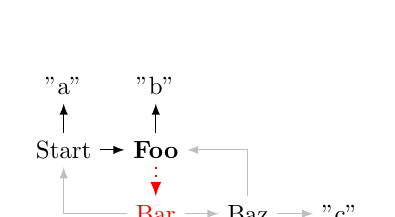
\begin{tikzpicture}[node distance=0.9cm, every node/.style={scale=0.9}]
		\node (end1) {"a"};
		\node (start) [below of=end1] {Start};
		\node (foo) [right of=start, xshift=0.4cm] {\textbf{Foo}};
		\node (end2) [above of=foo] {"b"};
		\node (bar) [below of=foo, text=red] {Bar};
		\node (baz) [right of=bar, xshift=0.4cm] {Baz};
		\node (end3) [right of=baz, xshift=0.4cm] {"c"};

		\draw [arrow] (start) -- (end1);
		\draw [arrow] (start) -- (foo);
		\draw [arrow] (foo) -- (end2);
		\draw [arrow, thick, dotted, red] (foo) -- (bar);
		\draw [arrow, lightgray] (bar) -| (start);
		\draw [arrow, lightgray] (bar) -- (baz);
		\draw [arrow, lightgray] (baz) |- (foo);
		\draw [arrow, lightgray] (baz) -- (end3);
	\end{tikzpicture}

	\caption{Pruning \ttfamily foo $\rightarrow$ bar}
	\label{fig:ringentryex2}
\end{figure}

As these examples illustrate, a head-first approach is prone to premature amputation of the grammar. Consequently, we discard this approach in favor of the one recommended in this paper for cheapening a grammar.

In the paradigm of a \textbf{tail-first} approach, the true cause of a ring is not the entry point but rather the 're-entry' point—the point at which the expansion path loops back onto itself. It is only at this point that the ring is formed.

Unlike the permissive and head-first approaches, where the operative entity is a rule, the operative entity of a tail-first approach is a pathway. Instead of saying "\verb|start| is recursive", we state "\verb|bar| $\rightarrow$ \verb|start| makes \verb|start| $\rightarrow$ \verb|foo| $\rightarrow$ \verb|bar| $\rightarrow$ \verb|start| recursive". A tail first approach therefore requires a sequential evaluation of every expansion path from \verb|start|.

Consider the simple example of a tail-first evaluation in action, in Figure \ref{fig:tlfstevalex}. Using this approach, we flag blameful rules, and simply filter them out when creating a copy of the original grammar.

\begin{figure}[hbt!]
	\centering

	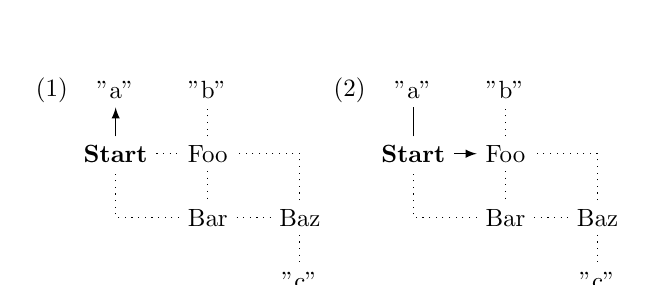
\begin{tikzpicture}[node distance=0.9cm, every node/.style={scale=0.9}]
		\node (1enum) {(1)};
		\node (1end1) [right of=1enum] {"a"};
		\node (1start) [below of=1end1] {\textbf{Start}};
		\node (1foo) [right of=1start, xshift=0.4cm] {Foo};
		\node (1end2) [above of=1foo] {"b"};
		\node (1bar) [below of=1foo] {Bar};
		\node (1baz) [right of=1bar, xshift=0.4cm] {Baz};
		\node (1end3) [below of=1baz] {"c"};

		\draw [arrow] (1start) -- (1end1);
		\draw [dotted] (1start) -- (1foo);
		\draw [dotted] (1foo) -- (1end2);
		\draw [dotted] (1foo) -- (1bar);
		\draw [dotted] (1bar) -| (1start);
		\draw [dotted] (1bar) -- (1baz);
		\draw [dotted] (1baz) |- (1foo);
		\draw [dotted] (1baz) -- (1end3);

		\node (2start) [right of=1foo, xshift=2cm] {\textbf{Start}};
		\node (2end1) [above of=2start] {"a"};
		\node (2enum) [left of=2end1] {(2)};
		\node (2foo) [right of=2start, xshift=0.4cm] {Foo};
		\node (2end2) [above of=2foo] {"b"};
		\node (2bar) [below of=2foo] {Bar};
		\node (2baz) [right of=2bar, xshift=0.4cm] {Baz};
		\node (2end3) [below of=2baz] {"c"};

		\draw (2start) -- (2end1);
		\draw [arrow] (2start) -- (2foo);
		\draw [dotted] (2foo) -- (2end2);
		\draw [dotted] (2foo) -- (2bar);
		\draw [dotted] (2bar) -| (2start);
		\draw [dotted] (2bar) -- (2baz);
		\draw [dotted] (2baz) |- (2foo);
		\draw [dotted] (2baz) -- (2end3);
	\end{tikzpicture}

	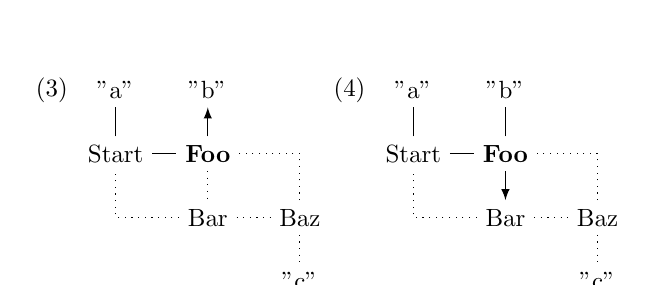
\begin{tikzpicture}[node distance=0.9cm, every node/.style={scale=0.9}]
		\node (1enum) {(3)};
		\node (1end1) [right of=1enum] {"a"};
		\node (1start) [below of=1end1] {Start};
		\node (1foo) [right of=1start, xshift=0.4cm] {\textbf{Foo}};
		\node (1end2) [above of=1foo] {"b"};1
		\node (1bar) [below of=1foo] {Bar};
		\node (1baz) [right of=1bar, xshift=0.4cm] {Baz};
		\node (1end3) [below of=1baz] {"c"};

		\draw (1start) -- (1end1);
		\draw (1start) -- (1foo);
		\draw [arrow] (1foo) -- (1end2);
		\draw [dotted] (1foo) -- (1bar);
		\draw [dotted] (1bar) -| (1start);
		\draw [dotted] (1bar) -- (1baz);
		\draw [dotted] (1baz) |- (1foo);
		\draw [dotted] (1baz) -- (1end3);

		\node (2start) [right of=1foo, xshift=2cm] {Start};
		\node (2end1) [above of=2start] {"a"};
		\node (2enum) [left of=2end1] {(4)};
		\node (2foo) [right of=2start, xshift=0.4cm] {\textbf{Foo}};
		\node (2end2) [above of=2foo] {"b"};
		\node (2bar) [below of=2foo] {Bar};
		\node (2baz) [right of=2bar, xshift=0.4cm] {Baz};
		\node (2end3) [below of=2baz] {"c"};

		\draw (2start) -- (2end1);
		\draw (2start) -- (2foo);
		\draw (2foo) -- (2end2);
		\draw [arrow] (2foo) -- (2bar);
		\draw [dotted] (2bar) -| (2start);
		\draw [dotted] (2bar) -- (2baz);
		\draw [dotted] (2baz) |- (2foo);
		\draw [dotted] (2baz) -- (2end3);
	\end{tikzpicture}

	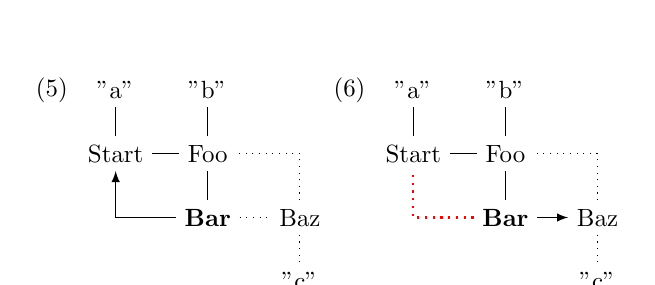
\begin{tikzpicture}[node distance=0.9cm, every node/.style={scale=0.9}]
		\node (1enum) {(5)};
		\node (1end1) [right of=1enum] {"a"};
		\node (1start) [below of=1end1] {Start};
		\node (1foo) [right of=1start, xshift=0.4cm] {Foo};
		\node (1end2) [above of=1foo] {"b"};
		\node (1bar) [below of=1foo] {\textbf{Bar}};
		\node (1baz) [right of=1bar, xshift=0.4cm] {Baz};
		\node (1end3) [below of=1baz] {"c"};

		\draw (1start) -- (1end1);
		\draw (1start) -- (1foo);
		\draw (1foo) -- (1end2);
		\draw (1foo) -- (1bar);
		\draw [arrow] (1bar) -| (1start);
		\draw [dotted] (1bar) -- (1baz);
		\draw [dotted] (1baz) |- (1foo);
		\draw [dotted] (1baz) -- (1end3);

		\node (2start) [right of=1foo, xshift=2cm] {Start};
		\node (2end1) [above of=2start] {"a"};
		\node (2enum) [left of=2end1] {(6)};
		\node (2foo) [right of=2start, xshift=0.4cm] {Foo};
		\node (2end2) [above of=2foo] {"b"};
		\node (2bar) [below of=2foo] {\textbf{Bar}};
		\node (2baz) [right of=2bar, xshift=0.4cm] {Baz};
		\node (2end3) [below of=2baz] {"c"};

		\draw (2start) -- (2end1);
		\draw (2start) -- (2foo);
		\draw (2foo) -- (2end2);
		\draw (2foo) -- (2bar);
		\draw [thick, dotted, red] (2bar) -| (2start);
		\draw [arrow] (2bar) -- (2baz);
		\draw [dotted] (2baz) |- (2foo);
		\draw [dotted] (2baz) -- (2end3);
	\end{tikzpicture}

	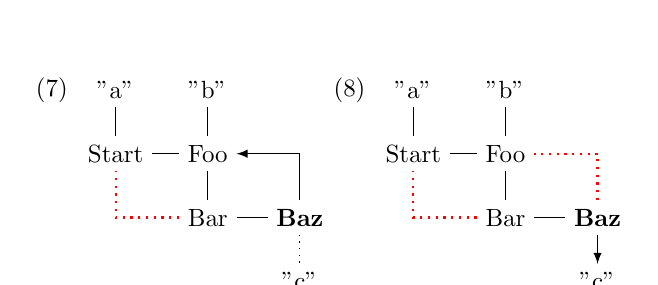
\begin{tikzpicture}[node distance=0.9cm, every node/.style={scale=0.9}]
		\node (1enum) {(7)};
		\node (1end1) [right of=1enum] {"a"};
		\node (1start) [below of=1end1] {Start};
		\node (1foo) [right of=1start, xshift=0.4cm] {Foo};
		\node (1end2) [above of=1foo] {"b"};
		\node (1bar) [below of=1foo] {Bar};
		\node (1baz) [right of=1bar, xshift=0.4cm] {\textbf{Baz}};
		\node (1end3) [below of=1baz] {"c"};

		\draw (1start) -- (1end1);
		\draw (1start) -- (1foo);
		\draw (1foo) -- (1end2);
		\draw (1foo) -- (1bar);
		\draw [thick, dotted, red] (1bar) -| (1start);
		\draw (1bar) -- (1baz);
		\draw [arrow] (1baz) |- (1foo);
		\draw [dotted] (1baz) -- (1end3);

		\node (2start) [right of=1foo, xshift=2cm] {Start};
		\node (2end1) [above of=2start] {"a"};
		\node (2enum) [left of=2end1] {(8)};
		\node (2foo) [right of=2start, xshift=0.4cm] {Foo};
		\node (2end2) [above of=2foo] {"b"};
		\node (2bar) [below of=2foo] {Bar};
		\node (2baz) [right of=2bar, xshift=0.4cm] {\textbf{Baz}};
		\node (2end3) [below of=2baz] {"c"};

		\draw (2start) -- (2end1);
		\draw (2start) -- (2foo);
		\draw (2foo) -- (2end2);
		\draw (2foo) -- (2bar);
		\draw [thick, dotted, red] (2bar) -| (2start);
		\draw (2bar) -- (2baz);
		\draw [thick, dotted, red] (2baz) |- (2foo);
		\draw [arrow] (2baz) -- (2end3);
	\end{tikzpicture}

	\caption{Tail-first evaluation of perfidious grammar}
	\label{fig:tlfstevalex}
\end{figure}

\subsubsection{Cheapening Implementation}

As discussed in the previous section:

\begin{quotation}
	\noindent A tail first approach [...] requires a sequential evaluation of every expansion path from \verb|start|.
\end{quotation}

We will therefore begin by creating a function that traverses every expansion path from \verb|start|. The approach is straightforward: for a given nonterminal, obtain the list of rules in the corresponding definition, and for each rule, generate a recursive call to the traversal function for every token in the rule:

\begin{lstlisting}[gobble=2, language=Python, caption={Grammar traversal}] 
	def flag(grammar, key="<start>"):
		for rule in grammar[key]:
			nonterms = set(nonterminals(rule))
				
			for token in nonterms:
				flag(grammar, token)
\end{lstlisting}

We also convert the list of nonterminals in a given rule into a set of unique values, to avoid redundant traversal. 

To identify when a expansion path loops back onto itself, we must maintain a path-specific history. Since this is a recursive traversal, this is once again as trivial as inheriting a parameter:

\begin{lstlisting}[gobble=2, language=Python, caption={Visited state}] 
	def flag(grammar, key="<start>", visited=["<start>"]):
		for rule in grammar[key]:
			nonterms = set(nonterminals(rule))
				
			for tkn in nonterms:
				flag(grammar, tkn, visited.copy() + [token])

\end{lstlisting}

Note the \verb|copy()| method used when passing the \verb|visited| to recursive sub-calls - this is to ensure the visited state is unique to each pathway, as Python by default passes lists by reference.

The final step is to actually identify a re-entry/loopback point and flag the offending rule. This is done simply by checking if any of the nonterminals in a given rule have previously been visited in the current expansion path:

\begin{lstlisting}[gobble=2, language=Python, caption={Flagging re-entry points}] 
	def flag(grammar, key="<start>", visited=["<start>"], flagged=[]):
		for rule in grammar[key]:
			if f"{key, rule}" not in flagged:
				nonterms = set(nonterminals(rule))

				# if loopback, flag rule
				if set(nonterms).intersection(set(visited)):
					flagged.append(f"{key, rule}")
				
				else: # otherwise continue traversal 
					for token in nonterms:
						flag(grammar, token, visited.copy() + [token], flagged)

		return flagged
\end{lstlisting}

You will notice that \verb|copy()| is not used when inheriting \verb|flagged| - this is because the list of flagged rules is not specific to an expansion path, and so passing by reference (ie. sharing the list between all recursive calls to \verb|flag()|) is desired behavior in this case.

To cheapen a grammar, \verb|flag()| is used to identify recursive re-entry points, and the original grammar is simply duplicated leaving out any rules present in the output of \verb|flag()|.

\subsection{Recursive Compiled Fuzzer}

We will now discuss the compiled output of a compiler that generates a recursive fuzzer. 

\subsubsection{Definitions to Generator Functions}

Going from the pseudocode presented in Section \ref{sec:genpsimp} to actual C program code for a definition is fairly trivial:

\begin{lstlisting}[gobble=2, language=C, caption={Recursive compiled fuzzer snippet}\label{lst:rcrcomfuz}]
	// cheap variant
	void expr_cheap() {
		switch (rand() % 1) {
			case 0:
				term_cheap();
				return;
		}
	}

	// random variant
	void expr_rand(int max_depth, int depth) {
		if (depth >= max_depth) { // redirect to cheap
			expr_cheap();
			return;
		}

		switch (rand() % 3) {
			case 0:
				term_rand(max_depth, depth + 1);
				return;
			
			case 1:
				term_rand(max_depth, depth + 1);
				putchar(43);
				expr_rand(max_depth, depth + 1);
				return;

			case 2:
				term_rand(max_depth, depth + 1);
				putchar(45);
				expr_rand(max_depth, depth + 1);
				return;
		}
	}
\end{lstlisting}

Each definition in a grammar will bee compiled as shown above and written to a file (e.g. \verb|core.c|). 

\subsubsection{Generating the Initiator}

We will also need to generate and include a main \verb|fuzz| function that will begin the fuzzing process - this will be common to any grammar:

\begin{lstlisting}[gobble=2, language=C, caption={Recursive compiled fuzzer initiator}]
	void fuzz(int seed, int max_depth) {
		// initialize random generator
		srand((unsigned) seed);

		gen_start_rand(max_depth, 0);
	}
\end{lstlisting}

This completes the compiled recursive fuzzer.

\subsection{Seeding (Interlude)}

You will have noticed the introduction of a \verb|seed| parameter to initialize the random generator in the previous section. This is not exclusive to compiled fuzzers - the random generator of a generic fuzzer is initialized in the \verb|main()| function where the \verb|fuzzer()| function is called. 

Due to the homologous approaches (Section \ref{sec:comapp}) to fuzzing the fuzzer variants presented in this paper follow, passing the same seed to any variant will result in each fuzzer producing the same fuzzed output.

\subsection{Iterative Compiled Fuzzer}

The iterative fuzzer is a hybrid between the generic iterative fuzzer and the compiled recursive fuzzer in that while it maintains an expansion stack that it continually evaluates the head of, expansions are still sub-calls (albeit not recursive), allowing us to borrow the simple depth state maintenance mechanism from the recursive fuzzer.

Unlike the generic iterative fuzzer, however, the stack stores function calls complete with arguments, a design choice influenced by the compilation of definitions into generator functions outlined in previous sections.

\subsubsection{Generating the Driver}

We will begin this time by generating the driver function:

\begin{lstlisting}[gobble=2, language=C, caption={Iterative compiled fuzzer driver}]
	Lambda stack[1024];
	int stack_len = 1;

	void fuzz(int seed, int max_depth) {
		// initialize random generator
		srand((unsigned) seed);

		// initialize stack with call to start generator
		stack[0] = (Lambda) {.args={max_depth, 0}, .func=&gen_start_rand};
		
		// execute first call in stack until stack is empty
		while (stack_len > 0) stack[0].func(stack[0].args[0], stack[0].args[1]);

		return;
	}
\end{lstlisting}

\verb|stack| and \verb|stack_len| are declared with global scope so that they may be later accessed by generator functions. 

\subsubsection{Lambda Functions}

You will notice that the stack is of type \verb|Lambda|. This is a structure we have created for the purpose of storing function calls in the stack, comprised of a function pointer, and an argument array. Listing \ref{lst:lambdastruct} shows the implementation of the structure, found in the header file generated by the compiler.

\begin{lstlisting}[gobble=2, language=C, caption={C Lambda Structure}, label=lst:lambdastruct]
	typedef void (*func)();

	typedef struct Lambda {
		int args[2];
		func func;
	} Lambda;
\end{lstlisting}

Calling and creating a lambda are both demonstrated in the driver code in the previous section.

\subsubsection{Definitions to Generator Functions}

The compilation of definitions is very similar to that of the recursive compiled fuzzer, with one main modification - instead of directly calling the subsequent generator functions present in the chosen rule, we prepend them to the expansion stack similarly to the generic iterative fuzzer. 

Consider Listing \ref{lst:itercompfuzzrule}, showing this modification made to a rule from the recursive compiled fuzzer in Listing \ref{lst:rcrcomfuz} (lines 23-26):

\begin{lstlisting}[gobble=2, language=C, caption={Iterative compiled fuzzer rule}, label=lst:itercompfuzzrule]
	// shift stack up to make space for expansion
	memmove(&stack[3], &stack[1], stack_len * sizeof(Lambda));
	
	// write function calls into space created
	stack[0] = (Lambda) {.args={max_depth, depth + 1}, .func=&gen_term_rand};

	stack[1] = (Lambda) {.args={43}, .func=&write};
	
	stack[2] = (Lambda) {.args={max_depth, depth + 1}, .func=&gen_expr_rand};
	
	stack_len += 2;
	return;
\end{lstlisting} 

\subsubsection{Handling Nonterminals}

The iterative compiled fuzzer, as you may have noticed in previous section's code, requires us to create a custom \verb|write()| function to handle terminals. Where the recursive variant allowed us to simply use \verb|putchar()|, additional stack operations in the iterative variant require a wrapper:

\begin{lstlisting}[gobble=2, language=C, caption={Custom write function}]
	void write(int token) {
		// remove call from stack
		memmove(&stack[0], &stack[1], stack_len * sizeof(Lambda));
		
		// write to stdout
		putchar(token);
		
		stack_len += -1;
		return;
	}
\end{lstlisting}

This completes the compiled iterative fuzzer.

\section{Profiling} \label{sec:profiling}

Fuzzer variants of each class (generic/compiled) and subtype (recursive/iterative) were generated for the JSON, TinyC, and HTTP grammars. To profile each variant, the corresponding executable was run for seed values $x$ such that  $\forall x\ 0 < x \leq 5000, x \in \mathbb{Z}$. Each data point is the average throughput of 10 runs of the fuzzer for the corresponding seed value $x$. The max depth argument for each execution is set to 128.

\subsection{Fuzzer Behavior}

Figures \ref{fig:json_size_vs_throughput_plot} through \ref{fig:http_size_vs_throughput_plot} plot raw profiling data for the compiled recursive fuzzers. The purpose of these figures is to visualize the behavior of all fuzzer variants for a given grammar - specifically in terms of throughput and output size. 

\textit{Note: The behavior of each fuzzer class and subtype was observed to be identical for a given grammar, and as such we have chosen to include visualizations for only the compiled recursive variants.}

\begin{figure}[hbt!]
	\centering

	\begin{tikzpicture}
		\begin{axis}[xlabel={Size (Kb)}, ylabel={Throughput (Kb/s)}, only marks, mark=., mark size=0.1pt]
			\addplot+[black] table [col sep=comma, x=Size (Kb), y=Throughput (Kb/s)] {profiling/cr_json.csv};
		\end{axis}
	\end{tikzpicture}
	
	\caption{Compiled recursive JSON fuzzer - Size vs. Throughput}
	\label{fig:json_size_vs_throughput_plot}
\end{figure}

\begin{figure}[hbt!]
	\centering

	\begin{tikzpicture}
		\begin{axis}[xlabel={Size (Kb)}, ylabel={Throughput (Kb/s)}, only marks, mark=., mark size=0.1pt]
			\addplot+[black] table [col sep=comma, x=Size (Kb), y=Throughput (Kb/s)] {profiling/cr_tinyc.csv};
		\end{axis}
	\end{tikzpicture}
	
	\caption{Compiled recursive TinyC fuzzer - Size vs. Throughput}
	\label{fig:tinyc_size_vs_throughput_plot}
\end{figure}

\begin{figure}[hbt!]
	\centering

	\begin{tikzpicture}
		\begin{axis}[xlabel={Size (Kb)}, ylabel={Throughput (Kb/s)}, only marks, mark=., mark size=0.1pt]
			\addplot+[black] table [col sep=comma, x=Size (Kb), y=Throughput (Kb/s)] {profiling/cr_http.csv};
		\end{axis}
	\end{tikzpicture}
	
	\caption{Compiled recursive HTTP fuzzer - Size vs. Throughput}
	\label{fig:http_size_vs_throughput_plot}
\end{figure}

Cursory analysis of the raw profiling data shows a drastically differing behavior profile for the TinyC grammar (Figure \ref{fig:tinyc_size_vs_throughput_plot}). We start by noting the possible correlation with average output size - $2.44 \cdot 10^{-1} < 6.45 \cdot 10^2 >> 5.89 \cdot 10^{-4}$ for JSON, TinyC, and HTTP respectively. 

We then conjecture then that the TinyC plot (Figure \ref{fig:tinyc_size_vs_throughput_plot}) visualizes the "complete" behavior profile of the fuzzers in this paper, or conversely that the JSON and HTTP behavior profiles are simply a subset of the more expansive (on the basis of output size size) TinyC profile. 

This is supported by Figure \ref{fig:tinyc_size_vs_throughput_plot_truncated}, which re-visualizes the behavior profile of the TinyC fuzzers by restricting output size to $<15$ kilobytes to approximate the output size range of the JSON fuzzer. We observe a distinct similarity between the truncated TinyC profile and the complete JSON profile - further limiting the visualization by an order of magnitude would likely yield a profile similar to the full HTTP profile.

\begin{figure}[hbt!]
	\centering

	\begin{tikzpicture}
		\begin{axis}[xlabel={Size (Kb)}, ylabel={Throughput (Kb/s)}, only marks, mark=., mark size=0.1pt]
			\addplot+[black] table [col sep=comma, x=Size (Kb), y=Throughput (Kb/s)] {profiling/cr_tinyc_truncated.csv};
		\end{axis}
	\end{tikzpicture}
	
	\caption{Compiled recursive TinyC fuzzer - Size vs. Throughput (truncated)}
	\label{fig:tinyc_size_vs_throughput_plot_truncated}
\end{figure}

In terms of the relationship between size and throughput, we also observe the following rough tendency:

\begin{equation} \label{eqn:size_throughput_trend}
	\lim_{\text{size}\to0} \text{throughput} \approx 0
\end{equation}

This suggests a lower limit on the execution time of the fuzzer that is independent of the output size, and is supported by the fact that each fuzzer variant profiled, regardless of grammar, had a minimum execution time $x$ such that $5 \cdot 10^{-4} < x < 6 \cdot 10^{-4}$.

\subsection{Benchmarking}

In consideration of the correlation described in (\ref{eqn:size_throughput_trend}), for comparative benchmarking of fuzzer variants we considered the average throughput of the ten largest fuzzed outputs for each fuzzer. Recall that all fuzzers achieve seeded output parity, meaning this selection is consistent across all variants for a given grammar. 

Figure \ref{fig:maximal_throughput_comparison} compares average maximal throughput for each fuzzer class/subtype, grouped by language. 

\begin{figure}[hbt!]
	\centering
	
	\pgfplotstableread[col sep=comma, header=true]{profiling/cumulative.csv}\datatable

	\begin{tikzpicture}
		\begin{axis}[ybar, bar width=0.3cm, xlabel={Language}, ylabel={Throughput}, ymax=25000,xtick=data, xticklabels from table={\datatable}{Language}, legend entries={Gen. Recursive, Gen. Iterative, Comp. Recursive, Comp. Iterative}, legend pos=north west, enlarge x limits={abs=1.5cm}, nodes near coords, every node near coord/.append style={rotate=90, anchor=west, font=\small}]
			\pgfplotsinvokeforeach{1,2,3,4}{\addplot table [x expr=\coordindex, y index=#1] {\datatable};}
		\end{axis}
	\end{tikzpicture}
	
	\caption{Maximal Throughput Comparison}
	\label{fig:maximal_throughput_comparison}
\end{figure}

We observe from the JSON and TinyC grammars that at large "enough" average output sizes, compiled fuzzers consistently outperform the generic class variants. We also observe that the performance difference between subtypes of the same class is far more prominent in generic fuzzers than compiled. 

The HTTP grammar, however, suggests that at low output sizes, all aforementioned differences become negligible (at least), with the generic variants slightly outperforming the compiled variants. 

\section{Discussion}

We have now successfully developed generic and compiled fuzzers with both iterative and recursive flow control that can efficiently generate fuzzed output given a JSON grammar. Comparing the maximal throughput we achieved for the JSON grammar with fuzzers described in this paper (5873.13 KB/s) with existing fast fuzzers for the same grammar\footnote{Generated from the ANTLR .g4 format JSON grammar (\url{https://raw.githubusercontent.com/antlr/grammars-v4/master/json/JSON.g4})} such as the F1 fuzzer \cite{Gopinath_2019} (4281.5 Kb/s), Grammarinator \cite{Hodovan_2018} (7 Kb/s), and an industry fuzzers such as Dharma by Mozilla \cite{Diehl_2014} (121.8 Kb/s), we find the performance of our fuzzers extremely adequate.

All in all, we have adequately demonstrated and designed fuzzers that are efficient in two ways - the first being in terms of raw throughput, and the second being in terms of \textit{valid} throughput, by virtue of being grammar fuzzers. The fuzzers we've developed allow us to quickly generate large (or, as large as the grammar is designed to allow) inputs in high volumes, greatly optimizing the input generation process of fuzz testing.

\section{Limitations and Future Work}

Approaching the end of the scope of this paper, we now discuss points of note that extend outside it that have a bearing on the usefulness of our results.

\subsection{Analysis}

With what limited analysis we performed on the fuzzers, we have identified a key bottleneck in the form of minimum execution time that leads to the throughput of any fuzzer to follow a plateau curve against size. We have roughly conjectured that the full extent of the behavior each fuzzer described in this paper follows this curve, or a subset of it, depending on the size distribution of its output. Further analysis of this with a larger number of grammars and a more powerful testing machine would likely give us more detailed insight into the behavior of the fuzzers and the cause of the lower-limit bottleneck respectively.

\subsection{Advanced Features}

The fuzzers developed in this paper are on the lower end of complexity as far as grammar fuzzers go. The fuzzers described herein may be further developed to add features such as individual probabilities for expansion rules, and depth control on a key-specific basis. This paper also assumes existing well-defined grammars for all use cases, whereas in actual application, we may instead be required to infer input grammars from sample input data corpora. These changes are likely required for the fuzzers to be considered for use in production or real testing.

\subsection{Grammar Cheapening}

The approach we have taken to cheapening grammars in this paper, while more efficient/less wasteful than alternative approaches we studied, is susceptible to creating dead-ends in grammars that contain definitions with no non-recursive rules. To minimally repopulate the cheap grammar such that no dead-ends are left we have, as an additional step, used the cheapening approach implemented in the F1 fuzzer \cite{Gopinath_2019} which assigns computational cost to each rule in a grammar, and chooses rules with minimum cost of all rules in a definition.

\section{Conclusion}

Fuzzing is a vastly useful technique in the process of security-testing software applications. Improvements in the speed of and control over fuzzed output generation could potentially optimize this process in a significant way; this paper has demonstrated how one might contribute to both areas of improvement; optimizing fuzzers by compiling fuzzers from grammar definitions - our fuzzers reach levels of throughput comparable to some of the faster fuzzers that currently exist - and by fuzzing from grammars to generate valid inputs much faster than a random fuzzer.

\bibliographystyle{apalike}
\bibliography{main}

\appendix

\section{Source Code \& Resources}

The source code and grammars for the fuzzers built in this paper are contained in \url{https://github.com/Positron11/fuzzer}. 

The G4 grammars that the JSON grammars were compiled from can be found at \url{https://github.com/antlr/grammars-v4/}. 

The tools used to perform the aforementioned compilation were provided by \url{https://github.com/vrthra/antlr2json/}

\end{document}
